% Copyright 2004 by Till Tantau <tantau@users.sourceforge.net>.
%
% In principle, this file can be redistributed and/or modified under
% the terms of the GNU Public License, version 2.
%
% However, this file is supposed to be a template to be modified
% for your own needs. For this reason, if you use this file as a
% template and not specifically distribute it as part of a another
% package/program, I grant the extra permission to freely copy and
% modify this file as you see fit and even to delete this copyright
% notice. 

\documentclass{beamer}
\usepackage{tikz}
\usetikzlibrary{trees}
\usepackage[ngerman]{babel}
\usepackage[utf8]{inputenc}
\usepackage{graphics}
\usetikzlibrary{positioning}
\usepackage[decimalsymbol=comma]{siunitx}
\usepackage{amsmath}
\usepackage{ziffer}
\usepackage{scrextend}
\usepackage{color, colortbl}
\usepackage{ulem}
\usepackage{multicol}
\usepackage{qrcode}


% There are many different themes available for Beamer. A comprehensive
% list with examples is given here:
% http://deic.uab.es/~iblanes/beamer_gallery/index_by_theme.html
% You can uncomment the themes below if you would like to use a different
% one:
%\usetheme{AnnArbor}
%\usetheme{Antibes}
%\usetheme{Bergen}
%\usetheme{Berkeley}
%\usetheme{Berlin}
%\usetheme{Boadilla}
%\usetheme{boxes}
%\usetheme{CambridgeUS}
%\usetheme{Copenhagen}
%\usetheme{Darmstadt}
\usetheme{default}
%\usetheme{Frankfurt}
%\usetheme{Goettingen}
%\usetheme{Hannover}
%\usetheme{Ilmenau}
%\usetheme{JuanLesPins}
%\usetheme{Luebeck}
%\usetheme{Madrid}
%\usetheme{Malmoe}
%\usetheme{Marburg}
%\usetheme{Montpellier}
%\usetheme{PaloAlto}
%\usetheme{Pittsburgh}
%\usetheme{Rochester}
%\usetheme{Singapore}
%\usetheme{Szeged}
%\usetheme{Warsaw}

\newcommand*\conj[1]{\overline{#1}}
\newcommand*\oo{\infty}

\definecolor{tucinfo}{rgb}{0.49,0.6,0.16}
\definecolor{LightCyan}{rgb}{0.88,1,1}
\definecolor{Blue}{rgb}{0,0,1}

\setbeamercolor{title}{fg=Blue}
\setbeamercolor{structure}{fg=Blue}


\title{cryptdomainmgr}

% A subtitle is optional and this may be deleted
\subtitle{automating Cert, TLSA, DKIM and many more}

\author{Stefan Helmert}
% - Give the names in the same order as the appear in the paper.
% - Use the \inst{?} command only if the authors have different
%   affiliation.

\institute[Entroserv] % (optional, but mostly needed)
{
	\url{https://www.entroserv.de/de/offene-software/cryptdomainmgr}
}


% - Use the \inst command only if there are several affiliations.
% - Keep it simple, no one is interested in your street address.

\date{20.04.2019}
%\date{\today}
% - Either use conference name or its abbreviation.
% - Not really informative to the audience, more for people (including
%   yourself) who are reading the slides online

\subject{Cryptdomainmgr}
% This is only inserted into the PDF information catalog. Can be left
% out. 

% If you have a file called "university-logo-filename.xxx", where xxx
% is a graphic format that can be processed by latex or pdflatex,
% resp., then you can add a logo as follows:

% \pgfdeclareimage[height=0.5cm]{university-logo}{university-logo-filename}
% \logo{\pgfuseimage{university-logo}}
\logo{\large{EH19}}

% Delete this, if you do not want the table of contents to pop up at
% the beginning of each subsection:
%\AtBeginSubsection[]
%{
%  \begin{frame}<beamer>{Inhalt}
%    \tableofcontents[currentsection,currentsubsection]
%  \end{frame}
%}

% Let's get started
\begin{document}
	
	\begin{frame}
		\titlepage
	\end{frame}
	
	\begin{frame}{Content}
		\begin{multicols}{2}
		\tableofcontents
		\end{multicols}
		% You might wish to add the option [pausesections]
	\end{frame}
	
	% Section and subsections will appear in the presentation overview
	% and table of contents.
	\pagenumbering{arabic}
	
	\section{Motivation}
	\begin{frame}{\insertsection}{\insertsubsection}
		\textbf{$\rightarrow$ let's make a web app $\leftarrow$}
		\begin{itemize}
			\item DNS
			\item Webpage
			\item E-Mail
			\item Mailinglist
			\item \textbf{and the s for security}
		\end{itemize}
	\end{frame}
	
	\section*{DeMotivation}
	\begin{frame}{\insertsection}{\insertsubsection}
		\vspace{-0.5cm}
		\textbf{$\rightarrow$ let's make a web app $\leftarrow$}
		\begin{itemize}
			\item DNS
			\begin{itemize}
				\item SOA
				\item DNSSEC
			\end{itemize}
			\item Webpage
			\begin{itemize}
				\item HTTPS
				\item Certificate
				\item HSTS
				\item SRV
				\item TLSA
			\end{itemize}
			\item E-Mail
			\begin{itemize}
				\item Spam
				\item DKIM
				\item SPF
				\item ADSP
				\item DMARC
				\item SRV
			\end{itemize}
			\item Mailinglist
			\begin{itemize}
				\item SRS
				\item ARC
			\end{itemize}
		\end{itemize}
	\end{frame}
	
	\subsection{fine}
	\begin{frame}{\insertsection}{\insertsubsection}
		\includegraphics[width=11cm]{CertOKen.png}
	\end{frame}

	\subsection{not so fine}
	\begin{frame}{\insertsection}{\insertsubsection}
		\includegraphics[height=8cm]{CertERRen.png}
	\end{frame}

	\section{Basics}
	\subsection{SSL Certifcate}
	\begin{frame}{\insertsection}{\insertsubsection}
		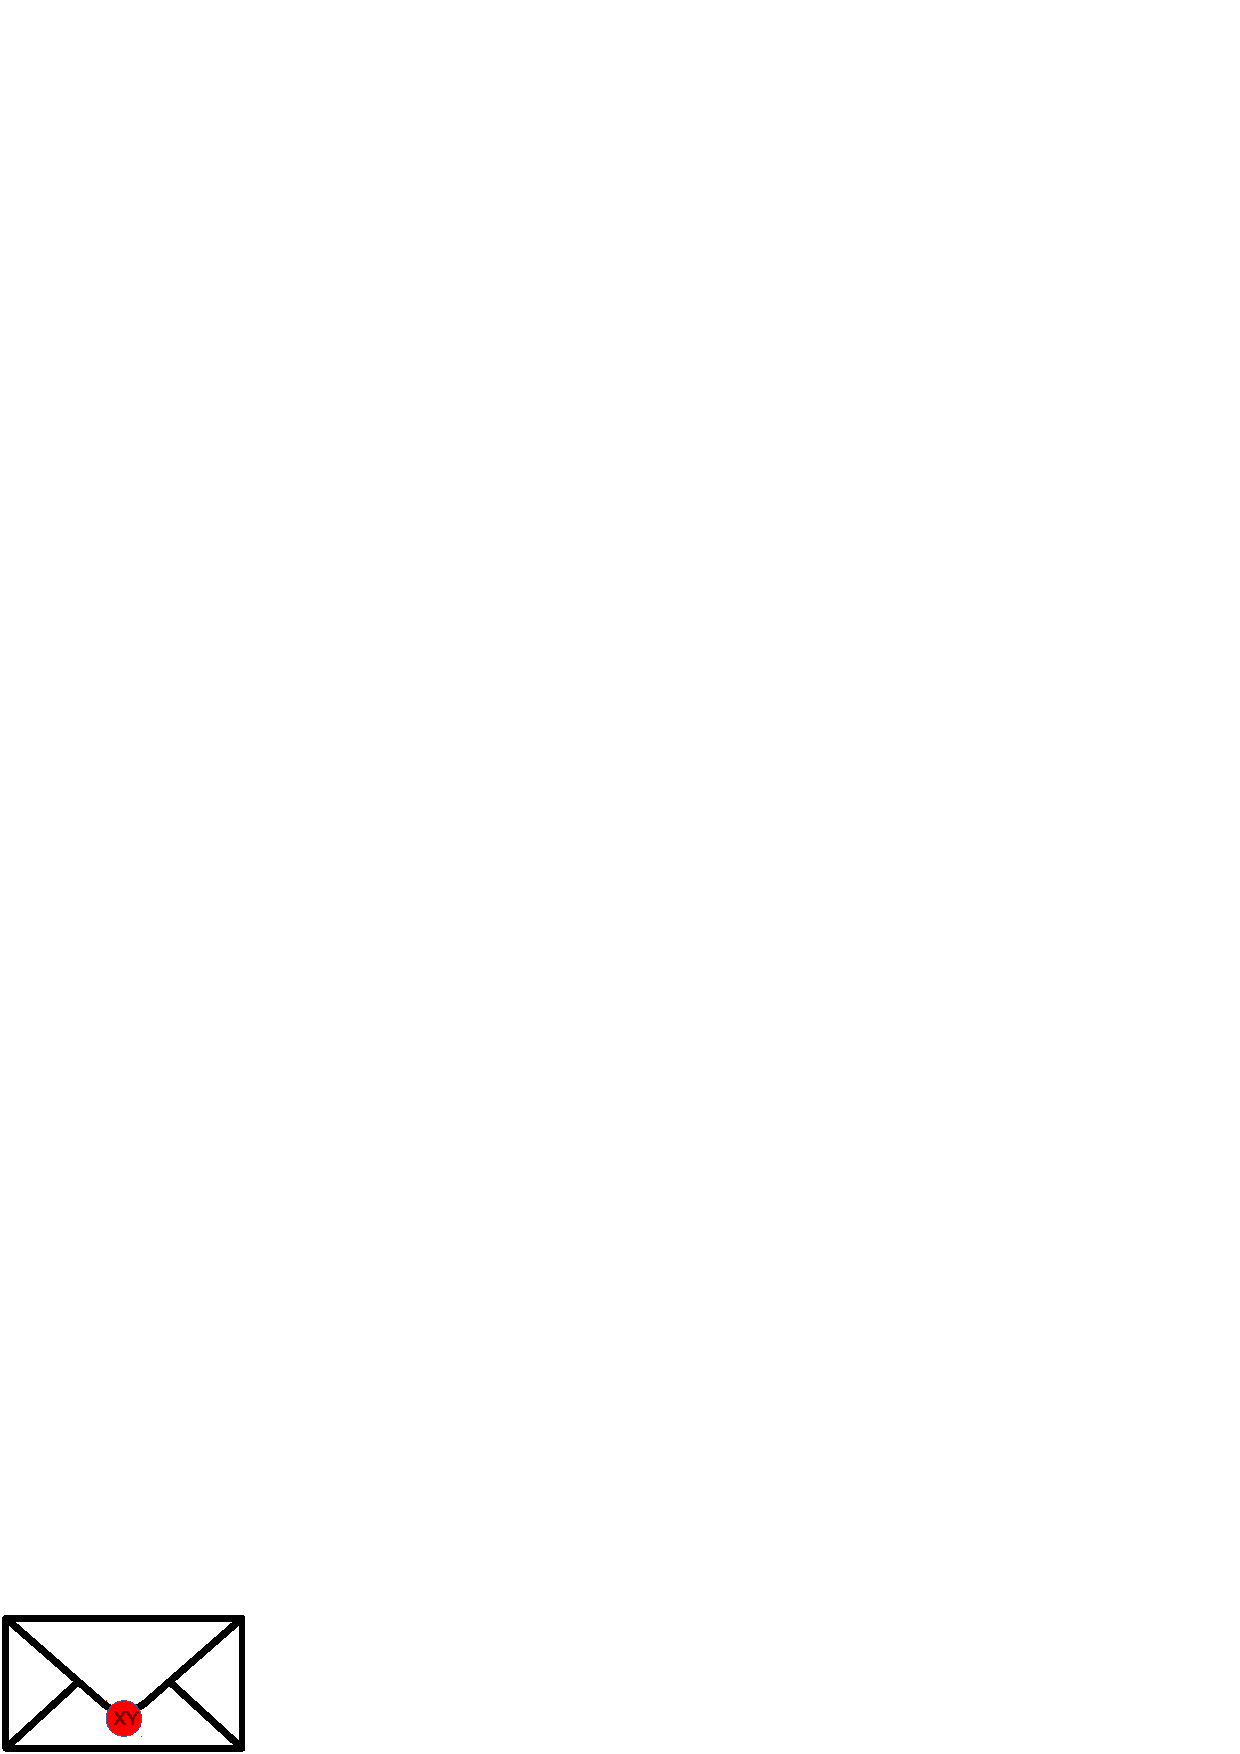
\includegraphics[height=3cm]{integrity.pdf}
		\begin{itemize}
			\item authentication (phishing)
			\item integrity (man in the middle)
			\item privacy (spy)
		\end{itemize}
		$\rightarrow$ certbot renew
	\end{frame}
	
	\subsection{TLSA}
	\begin{frame}{\insertsection}{\insertsubsection}
		\textbf{DANE -- DNS-based Authentication of Named Entities}\\		\includegraphics[height=3.8cm]{TLSA.pdf}\\
		\textbf{TLSA -- Transport Layer Security Authentication} 
		\begin{itemize}
			\item locks certificate to domain/DNS (fraudulent CA, stolen cert)
		\end{itemize}
		$\rightarrow$ to do \\
	\end{frame}	
	
	\subsection{CAA}
	\begin{frame}{\insertsection}{\insertsubsection}
		\includegraphics[height=4.5cm]{CAA.pdf}\\
		\textbf{CAA -- Certification Authority Authorization}
		\begin{itemize}
			\item specifies allowed CA
			\item checked by CA
		\end{itemize}
	\end{frame}	
	
	\subsection{DNSSEC}
	\begin{frame}{\insertsection}{\insertsubsection}
		\includegraphics[height=4cm]{DNSSEC.pdf}\\
		\textbf{Domain Name System Security Extensions} 
		\begin{itemize}
			\item authenticate domain owner
			\item integrity (DNS cache poisoning)
			\item proof of nonexistence
		\end{itemize}
		$\rightarrow$ done by domain provider
	\end{frame}
	
	\subsection{DANE -- all steps}
	\begin{frame}{\insertsection}{\insertsubsection}
		\includegraphics[width=11cm]{CertProcedure.pdf}\\
	\end{frame}	
	
	
	\subsection{MX}
	\begin{frame}{\insertsection}{\insertsubsection}
		\includegraphics[width=11cm]{MX.pdf}\\
		\textbf{Mail eXchange} 
		\begin{itemize}
			\item abstraction: email domain, email server domain
			\item multiple email servers
		\end{itemize}
	\end{frame}	

	\subsection{SPF}
	\begin{frame}{\insertsection}{\insertsubsection}
		\includegraphics[width=11cm]{MXrev.pdf}\\
		\textbf{MX backwards} 
		\begin{itemize}
			\item faked sender?
		\end{itemize}
	\end{frame}	

	\begin{frame}{\insertsection}{\insertsubsection}
		\includegraphics[width=11cm]{SPF.pdf}\\
		\textbf{SPF -- Sender Policy Framework} 
		\begin{itemize}
			\item MX alled to send
			\item no one else allowed
		\end{itemize}
	\end{frame}	
		
	\subsection{DKIM}
	\begin{frame}{\insertsection}{\insertsubsection}
		\includegraphics[height=4cm]{DKIM.pdf}\\
		\textbf{DomainKeys Identified Mail} 
		\begin{itemize}
			\item authenticate MTA (fake/spam server)
			\item integrity (man in the middle)
		\end{itemize}
		$\rightarrow$ to do
	\end{frame}

	\subsection{additional DNS records}
	\begin{frame}{\insertsection}{\insertsubsection}

		\textbf{SPF -- Sender Policy Framework} 
		\begin{itemize}
			\item which server is allowed to send email
		\end{itemize}
		\textbf{ADSP -- Author Domain Signing Practices}
		\begin{itemize}
			\item defines, if email must be DKIM signed
		\end{itemize}	
		\textbf{DMARC -- Domain-based Message Authentication, Reporting and Conformance}
		\begin{itemize}
			\item successor of SPF and ADSP
			\item overrides SPF and ADSP
			\item additional parameters: report email
		\end{itemize}
		\textbf{SRV -- Service}
		\begin{itemize}
			\item announces services
		\end{itemize}
	\end{frame}

	\subsection{DKIM -- overview}
	\begin{frame}{\insertsection}{\insertsubsection}
		\includegraphics[width=11.5cm]{DKIMProcedure.pdf}\\
	\end{frame}
		
	\section{Cryptdomainmgr}
	\subsection{dataflow}
	\begin{frame}{\insertsection}{\insertsubsection}
	\textbf{Infrastructure as Code!}\\ \bigskip
	\begin{tikzpicture}[
	invisiblenode/.style={minimum size=5mm},
	slidenode/.style={rectangle, draw=blue!60, fill=blue!5, very thick, minimum size=6mm},
	nonode/.style={circle, fill=green!5, very thick, minimum size=7mm},
	roundnode/.style={circle, draw=red!60, fill=red!5, very thick, minimum size=11mm},
	squarednode/.style={rectangle, draw=red!60, fill=red!5, very thick, minimum size=5mm},
	]
	%Nodes
	\node[slidenode]    (slide1)                {DNS-Server};
	\node[slidenode]    (slide2) [right=of slide1]                  {Web-/Mailserver};	
	\node[slidenode]    (slide3) [right=of slide2]                  {CA};
	\node[squarednode] (neuron) [below=of slide2]                       {Cryptdomainmgr};	\node[invisiblenode]    (arl) [right=of neuron]               {};
	\node[nonode]    (out)    [below=of neuron]                    {Configuration};		\node[invisiblenode]    (arr) [right=of arl]               {};
	%Lines
	\draw[->] (slide3.south) .. controls +(down:10mm) and +(right:10mm) .. (neuron.east) node[midway,sloped] {\shortstack{\bigskip \\ Certificate}};
	\draw[<-] (slide2.south) -- (neuron.north)  node[rotate=90, midway,sloped] {\shortstack{Cert, DKIM}};
	\draw[<-] (slide1.south) .. controls +(down:10mm) and +(left:10mm) .. (neuron.west) node[midway,sloped] {\shortstack{\bigskip \\ Update Records}};	
	\draw[<-] (neuron.south) -- (out.north);
	\end{tikzpicture}		
	\end{frame}
		
	\subsection{autorenew process}
	\begin{frame}{\insertsection}{\insertsubsection}
		\begin{itemize}
			\item prepare
			\begin{itemize}
				\item generate certificate
				\item calculate TLSA from certificate
				\item add TLSA RR
				\item generate key pair for DKIM
				\item calculate DKIM
				\item add DKIM RR
			\end{itemize}
			\item rollover
			\begin{itemize}
				\item use new certificate
				\item use new DKIM key
			\end{itemize}
			\item cleanup
			\begin{itemize}
				\item remove old TLSA RR
				\item remove old DKIM RR
				\item delete old certificates
				\item delete old DKIM keys		
			\end{itemize}
		\end{itemize}
	\end{frame}
	

\subsection{structure}
\begin{frame}{\insertsection}{\insertsubsection}
\tikzstyle{every node}=[draw=orange,fill=orange!20,thick,anchor=west]
\tikzstyle{root}=[draw=white,fill=blue!10]
\tikzstyle{none}=[draw=white,fill=white]
\tikzstyle{file}=[draw=black,fill=white]
\begin{tikzpicture}[%
grow via three points={one child at (0.5,-0.7) and
	two children at (0.5,-0.7) and (0.5,-1.4)},
edge from parent path={(\tikzparentnode.south) |- (\tikzchildnode.west)}]
\node [root] {cryptdomainmgr}
child { node [file] {\_\_main\_\_.py}}	
child { node [file] {\_\_init\_\_.py}}			
child { node {modules}
	child { node [none] {...}}	
}
child [missing] {}				
child { node [file] {cdmcore.py}}
child { node [file] {cdmstatehandler.py}}								
child { node [file] {cdmconfighandler.py}};
\end{tikzpicture}
\end{frame}	
	
\begin{frame}{\insertsection}{\insertsubsection}
	\tikzstyle{every node}=[draw=orange,fill=orange!20,thick,anchor=west]
	\tikzstyle{root}=[draw=white,fill=blue!10]
	\tikzstyle{none}=[draw=white,fill=white]
	\tikzstyle{file}=[draw=black,fill=white]
	\begin{tikzpicture}[%
	grow via three points={one child at (0.5,-0.7) and
		two children at (0.5,-0.7) and (0.5,-1.4)},
	edge from parent path={(\tikzparentnode.south) |- (\tikzchildnode.west)}]
	\node [root] {cryptdomainmgr}	
	child { node [none] {...}}
	child { node {modules}
		child { node {common}}
		child { node {cdm}}
		child { node {cert}}
		child { node {dkim}}
		child { node {domain}}
		child { node {service}}
		child { node {dhparam}}
	};
	\end{tikzpicture}
\end{frame}	
	
\begin{frame}{\insertsection}{\insertsubsection}
	\tikzstyle{every node}=[draw=orange,fill=orange!20,thick,anchor=west]
	\tikzstyle{dirdot}=[draw=white,fill=orange!20,thick,anchor=west]
	\tikzstyle{root}=[draw=white,fill=blue!10]
	\tikzstyle{none}=[draw=white,fill=white]
	\tikzstyle{file}=[draw=black,fill=white]
	\begin{tikzpicture}[%
	grow via three points={one child at (0.5,-0.7) and
		two children at (0.5,-0.7) and (0.5,-1.4)},
	edge from parent path={(\tikzparentnode.south) |- (\tikzchildnode.west)}]
	\node [root] {cryptdomainmgr}	
	child { node [none] {...}}
	child { node {modules}
		child { node [dirdot] {...}}
		child { node {domain}
			child { node [file] {\_\_init\_\_.py}}		
			child { node [file] {main.py}}		
			child { node [file] {confighandler.py}}		
			child { node [file] {handlerdnsuptools.py}}		
		}
	};
	\end{tikzpicture}
\end{frame}	

\section{Usage}
\begin{frame}[fragile]{\insertsection}{\insertsubsection} % fragiel: no indentation allowed
	\url{www.entroserv.de/de/offene-software/cryptdomainmgr}\\
	\qrcode{www.entroserv.de/de/offene-software/cryptdomainmgr}
\end{frame}		

\subsection{update cycle}
\begin{frame}[fragile]{\insertsection}{\insertsubsection} % fragiel: no indentation allowed
	\textbf{update -- set static entries: a, aaaa, srv, dmarc, spf, adsp}
	\begin{verbatim}
	$ python -m cryptdomainmgr --update cred.cnf exmpl.cnf
	\end{verbatim}
	\vspace{0.3cm}
	
	\textbf{prepare, rollover, cleanup cycle -- renew cryptographic material: certificate, TLSA, DKIM}
	\begin{verbatim}
	$ python -m cryptdomainmgr cred.cnf exmpl.cnf
	\end{verbatim}
	\vspace{0.3cm}
	\textbf{explicit cycle}
	\begin{verbatim}
	$ python -m cryptdomainmgr --prepare cred.cnf exmpl.cnf
	$ python -m cryptdomainmgr --rollover cred.cnf exmpl.cnf
	$ python -m cryptdomainmgr --cleanup cred.cnf exmpl.cnf
	\end{verbatim}
\end{frame}	

\subsection{DNS credential}
\begin{frame}[fragile]{\insertsection}{\insertsubsection} % fragile: no indentation allowed
	\begin{verbatim}
	$ cat cred.cnf
	
	[domain]
	user = myusername
	passwd = mypassword
	\end{verbatim}
\end{frame}		

\subsection{Certificates}
\begin{frame}[fragile]{\insertsection}{\insertsubsection} % fragile: no indentation allowed
	\begin{verbatim}
	$ cat exmpl.cnf
	
	[cert]
	handler = dehydrated
	email = stefan.helmert@t-online.de
	keysize = 4096
	
	[cert:maincert]
	destination = /etc/ssl
	extraflags = --staging, -x
	certname = fullchain.pem
	\end{verbatim}
	\begin{itemize}
		\item multiple domains using \texttt{maincert} $\rightarrow$ SAN certificate
	\end{itemize}
\end{frame}	

\subsection{DKIM}
\begin{frame}[fragile]{\insertsection}{\insertsubsection} % fragile: no indentation allowed
	\begin{verbatim}
	$ cat exmpl.cnf
	
	[dkim]
	handler = rspamd
	
	[dkim:maindkim]
	signingConfTemplateFile
	  = /etc/cryptdomainmgr/dkim_signing_template.conf
	signingConfDestinationFile
	  = /etc/rspamd/local.d/dkim_signing.conf
	\end{verbatim}
\end{frame}	
	
\subsection{Domain}
\begin{frame}[fragile]{\insertsection}{\insertsubsection} % fragile: no indentation allowed
	\begin{verbatim}
	$ cat exmpl.cnf
	
	[domain]
	user = myusername
	handler = dnsuptools/inwx
	
	[domain:domain.example]
	soa.hostmaster = stefan.helmert@t-online.de
	soa.refresh = 7200
	
	[domain:sub.domain.example]
	ip4 = auto, 192.168.0.1
	ip6+ = auto, 0ffc::0030
	mx = mail20.domain.example:20, mail30.domain.example:30
	mx.40 = mail40.domain.example, mail50.domain.example:50
	mx.10+= mail10.domain.example
	\end{verbatim}
\end{frame}	

\begin{frame}[fragile]{\insertsection}{\insertsubsection} % fragile: no indentation allowed
	\textbf{set A record}
	\begin{verbatim}
	$ cat exmpl.cnf
	
	[domain:sub.domain.example]
	ip4 = auto, 192.168.0.1
	\end{verbatim}
	means:
	\begin{itemize}
		\item add external ip and \texttt{192.168.0.1} to sub.domain.example
		\item delete all other A records of sub.domain.example
	\end{itemize}
\end{frame}	

\begin{frame}[fragile]{\insertsection}{\insertsubsection} % fragile: no indentation allowed
	\textbf{add A record}
	\begin{verbatim}
	$ cat exmpl.cnf
	
	[domain:sub.domain.example]
	ip4+ = auto, 192.168.0.1
	\end{verbatim}
	means:
	\begin{itemize}
		\item add external ip and \texttt{192.168.0.1} to sub.domain.example
		\item \sout{delete all other A records of sub.domain.example}
	\end{itemize}
\end{frame}	

\begin{frame}[fragile]{\insertsection}{\insertsubsection} % fragile: no indentation allowed
	\textbf{set MX record}
	\begin{verbatim}
	$ cat exmpl.cnf
		
	[domain:sub.domain.example]
	mx = mail20.domain.example:20, mail30.domain.example:30
	\end{verbatim}
	means:
	\begin{itemize}
		\item add MX records
		\begin{itemize}
			\item mail20.domain.example with prio 20
			\item mail30.domain.example with prio 30
		\end{itemize}
		\item delete all other MX records from sub.domain.example
	\end{itemize}
\end{frame}	

\begin{frame}[fragile]{\insertsection}{\insertsubsection} % fragile: no indentation allowed
	\textbf{set MX record}
	\begin{verbatim}
	$ cat exmpl.cnf
			
	[domain:sub.domain.example]
	mx.40 = mail40.domain.example, mail50.domain.example:50
	\end{verbatim}
	means:
	\begin{itemize}
		\item add MX records
		\begin{itemize}
			\item mail40.domain.example with prio 40
			\item mail50.domain.example with prio 50
		\end{itemize}
		\item delete all other MX records with prio 40 from sub.domain.example
	\end{itemize}	
\end{frame}	

\begin{frame}[fragile]{\insertsection}{\insertsubsection} % fragile: no indentation allowed
	\textbf{set SRV record}
	\begin{verbatim}
	$ cat exmpl.cnf
		
	[domain:sub.domain.example]
	srv.service.proto.port.weight.prio 
	  = sub.domain.example:PRIO:WEIGHT:PORT:PROTO:SERVICE
	\end{verbatim}
\end{frame}	

\begin{frame}[fragile]{\insertsection}{\insertsubsection} % fragile: no indentation allowed
	\textbf{set DMARC entries}
	\begin{verbatim}
	$ cat exmpl.cnf
		
	[domain:sub.domain.example]
	dmarc.p = quarantine
	dmarc.rua = mailto:stefan.helmert@t-online.de
	dmarc.ruf = mailto:stefan.helmert@gmx.net
	\end{verbatim}
	\begin{itemize}
		\item changes the entries \texttt{p}, \texttt{rua}, \texttt{ruf} of the \texttt{DMARC} record
		\item entries \texttt{adkim}, \texttt{aspf}, \texttt{pct} do not change
		\item "`atomic"' operation
		\item only one \texttt{DMARC} record allowed!
	\end{itemize}
\end{frame}	

\begin{frame}[fragile]{\insertsection}{\insertsubsection} % fragile: no indentation allowed
	\textbf{set DMARC record}
	\begin{verbatim}
	$ cat exmpl.cnf
		
	[domain:sub.domain.example]
	dmarc =
	dmarc.p = quarantine
	dmarc.rua = mailto:stefan.helmert@t-online.de
	dmarc.ruf = mailto:stefan.helmert@gmx.net
	\end{verbatim}
	\begin{itemize}
		\item changes the entries \texttt{p}, \texttt{rua}, \texttt{ruf} of the \texttt{DMARC} record
		\item remove all other entries of this record
		\item atomic operation
		\item at most one \texttt{DMARC} record allowed!
	\end{itemize}
\end{frame}	

\begin{frame}[fragile]{\insertsection}{\insertsubsection} % fragile: no indentation allowed
	\textbf{set SOA entries}
	\begin{verbatim}
	$ cat exmpl.cnf
		
	[domain:domain.example]
	soa.hostmaster = stefan.helmert@t-online.de
	soa.refresh = 7200
	\end{verbatim}
	\begin{itemize}
		\item changes the entries \texttt{hostmaster}, \texttt{refresh} of the \texttt{SOA} record
		\item \texttt{primns}, \texttt{serial}, \texttt{retry}, \texttt{expire}, \texttt{ncttl} not changed
		\item atomic operation
		\item exact one \texttt{SOA} record in top level allowed!
	\end{itemize}
\end{frame}	

\begin{frame}[fragile]{\insertsection}{\insertsubsection} % fragile: no indentation allowed
	\textbf{set SPF flags}
	\begin{verbatim}
	$ cat exmpl.cnf
		
	[domain:domain.example]
	spf = -mx, a, ?all, +aaaa
	\end{verbatim}
	\begin{itemize}
		\item add given flags to \texttt{SPF} record
		\item remove all other flags from \texttt{SPF} record
		\item atomic operation
		\item at most one \texttt{SPF} record is allowed!
	\end{itemize}
\end{frame}	

\begin{frame}[fragile]{\insertsection}{\insertsubsection} % fragile: no indentation allowed
	\textbf{set ADSP and CAA records}
	\begin{verbatim}
	$ cat exmpl.cnf
		
	[domain:domain.example]
	adsp = all
	caa =   0 issue letsdecrypt.org,
	      128 issuewild examplecert.example
	\end{verbatim}
	\begin{itemize}
		\item atomic update \texttt{ADSP} record
		\item add the \texttt{CAA} records
		\item remove all other \texttt{CAA} records
	\end{itemize}
	\textbf{configured by cert handler:} 
	\begin{verbatim}
	[domain:domain.example]
	caa =   auto 
	\end{verbatim}
\end{frame}	


\begin{frame}[fragile]{\insertsection}{\insertsubsection} % fragile: no indentation allowed
	\textbf{combine stuff -- TLSA and DKIM}
	\begin{verbatim}
	$ cat exmpl.cnf

	[domain:sub.domain.example]	
	tlsa.tcp.443 = auto:3:0:1, auto:2:0:1
	cert = maincert
	dkim = maindkim
	\end{verbatim}
	\textbf{prepare cycle}
	\begin{itemize}
		\item add \texttt{TLSA} and \texttt{DKIM} records
	\end{itemize}
	\textbf{rollover cycle}
	\begin{itemize}
		\item no DNS changes
		\item apply certificates and keys on server
	\end{itemize}	\textbf{cleanup cycle}
	\begin{itemize}
		\item add \texttt{TLSA} and \texttt{DKIM} records (again)
		\item remove all other \texttt{TLSA} and \texttt{DKIM} records
	\end{itemize}	
\end{frame}	

\section{Implementation}
\subsection{cryptdomainmgr}
\begin{frame}[fragile]{\insertsection}{\insertsubsection} % fragile: no indentation allowed
	\begin{description}
		\item[\_\_main\_\_.py] command line interface
		\item[cdmcore.py] core, brings everything together
		\item[cdmconfighandler.py] reads/interpretes config (ini) files
		\item[cdmstatehandler.py] manages dependencies, data transport, next run phase
		\item[modules/] plugins handling/interfacing dns update, certificate renewal, dkim renewal, service reload
	\end{description}
	
	\textbf{external packages:}
	\begin{description}
		\item[simpleloggerplus] logging abstraction, password $\rightarrow$ *****
		\item[dnsuptools] domrobot interface abstraction, TLSA, DKIM calculation
	\end{description}
\end{frame}	

	\begin{frame}{\insertsection}{\insertsubsection}
		\textbf{Reactive:} Domain update depends on TLSA record calculated based on new certificate. \\ \bigskip
		\begin{tikzpicture}[
		invisiblenode/.style={minimum size=5mm},
		slidenode/.style={rectangle, draw=blue!60, fill=blue!5, very thick, minimum size=6mm},
		nonode/.style={circle, fill=green!5, very thick, minimum size=7mm},
		roundnode/.style={circle, draw=red!60, fill=red!5, very thick, minimum size=11mm},
		squarednode/.style={rectangle, draw=red!60, fill=red!5, very thick, minimum size=5mm},
		dashednode/.style={rectangle, dashed, draw=red!60, fill=red!5, very thick, minimum size=5mm},
		]
		%Nodes
		\node[slidenode]    (cert)                {Certificate Update};
		\node[dashednode]    (wait) [below=of cert]               {Update Domain};
		\node[slidenode]    (domain) [right=of wait]                  {Update Domain};
		\node[invisiblenode]		(modcert) [left=of cert, text width=2.5cm] {\textbf{modules/cert}};
		\node[invisiblenode]		(moddomain) [below=of modcert, text width=2.5cm] {\textbf{modules/domain}};
		%Lines
		\draw[->] (cert.east) .. controls +(right:9mm) and +(left:9mm) .. (domain.west) node [midway,sloped, rotate=180] {\shortstack{\\ \bigskip TLSA}} ;
		\end{tikzpicture}		
	\end{frame}

\subsection{modules}
\begin{frame}[fragile]{\insertsection}{\insertsubsection} % fragile: no indentation allowed
	\begin{description}
		\item[modules/cert/main.py] interface to handler, some helpers
		\item[modules/cert/handlerdehydrated.py] interface todehydrated to create certificate
		\item[modules/cert/confighandler.py] interpretes corrspondig parts of the config file
	\end{description}
	\textbf{external package:}
	\begin{description}
		\item[dehydrated] handles acme api for letsencrypt
	\end{description}	

\end{frame}	

\subsection{simpleloggerplus} \label{sec:simpleloggerplus}
\begin{frame}[fragile]{\insertsection}{\insertsubsection} % fragile: no indentation allowed
	\begin{description}
		\item[simpleloggerplus.py] core, produces output
		\item[deepops.py] deep dict/list operations, password $\rightarrow$ *****
	\end{description}	
\end{frame}	

\subsection{dnsuptools}
\begin{frame}[fragile]{\insertsection}{\insertsubsection} % fragile: no indentation allowed
	\begin{description}
		\item[dnsuptools.py] core, high level, record change \& query methods
		\item[dnsupdate.py] interface to wrapper, low level
		\item[inwxwrapper.py] interface to internetworx api, lowest level
		\item[dkimrecgen.py] reads/interpretes dkim key file
		\item[tlsarecgen.py] reads/interpretes certificate file
		\item[dnshelpers.py] one helper function
	\end{description}
	\textbf{external packages:}	
	\begin{description}
		\item[simpleloggerplus] see simpleloggerplus \ref{sec:simpleloggerplus}
		\item[inwxclient] domrobot client
	\end{description}	
\end{frame}	

\section{Discussion}
\begin{frame}[fragile]{\insertsection}{\insertsubsection} % fragile: no indentation allowed
  \Huge{???}	
\end{frame}	

\end{document}





\grid
\grid
